%\documentclass[handout]{beamer} % set [handout] as an option to remove /pause breaks
\documentclass{beamer}
\usetheme{McMaster}
\beamertemplatenavigationsymbolsempty 
\usepackage{tikz}
\usepackage[export]{adjustbox} % for left/right justifying images
\title{AI workshop}
\date{Oct 23rd, 2024}

\begin{document}
\begin{frame}
	\maketitle
\end{frame}

\begin{frame}
	Why care about local?
\end{frame}

\begin{frame}
	\begin{itemize}
		\item Privacy
		\pause
		\item Environmental
		\pause
		\item Cost
	\end{itemize}
\end{frame}

\begin{frame}[plain]
	\makebox[\linewidth]{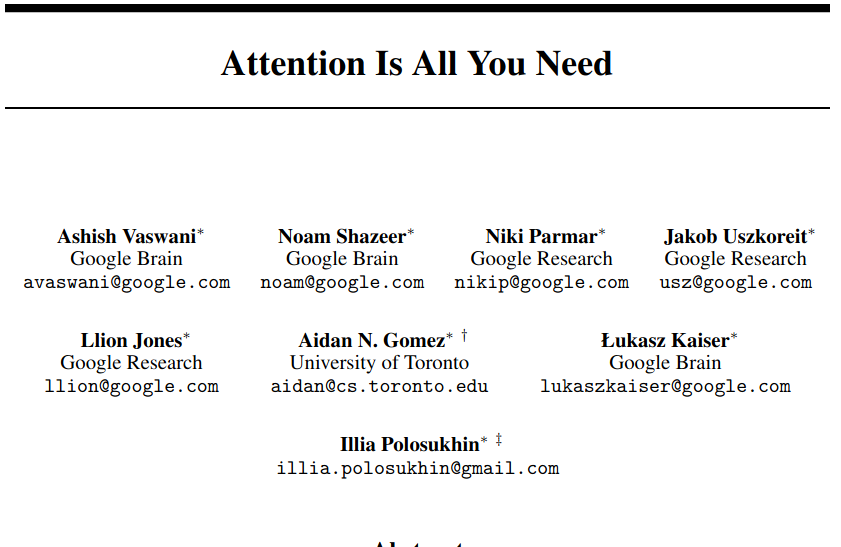
\includegraphics[width=\paperwidth,height=\paperheight]{images/attention}}
\end{frame}

\begin{frame}[plain]
	\makebox[\linewidth]{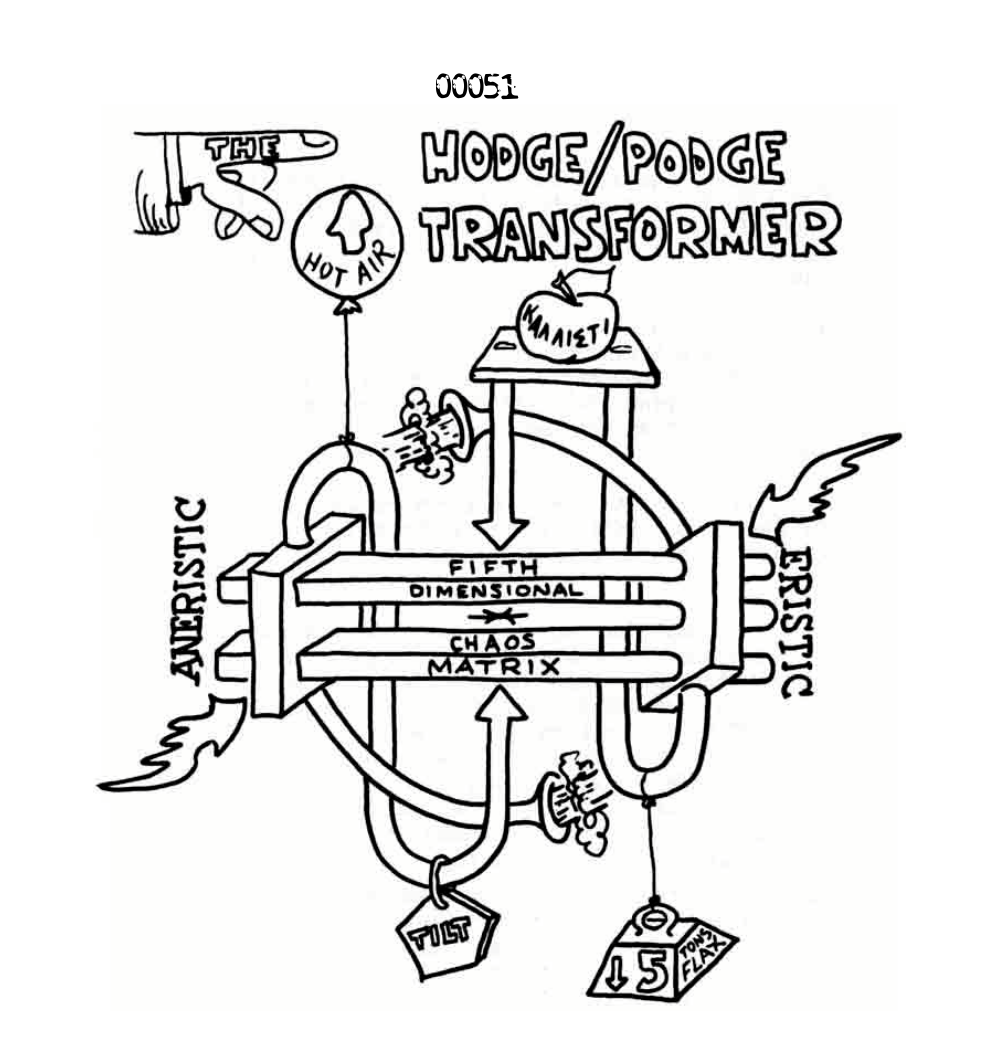
\includegraphics[width=\paperwidth,height=\paperheight]{images/hodge-podge}}
\end{frame}


\begin{frame}{Important concepts for transformer-based models}
	\begin{itemize}
		\item Context Window and Tokens
		% Has gone up enormously in the past year. Now GPT-4 has a max window of 128k, some open models have this or more.
		\pause
		\item Temperature
		\pause
		\item Parameters
		% GPT-1 117m, GPT-2 1.5b, GPT-3 175b, GPT-4 170t?
		\pause
		\item Training
		\pause 
		\item The Random Seed.
		\pause
		\item The Prompt, aka "Programming for English Majors"
	\end{itemize}
\end{frame}

\begin{frame}[plain]
	\makebox[\linewidth]{
\includegraphics[width=\paperwidth,height=\paperheight]{images/hottest-language}}
\end{frame}

\begin{frame}
	\begin{itemize}
		\item Context Window is the "memory" of an LLM
		\pause
		\item And Tokens -- words, roughly -- fill up that "memory"
		\pause
		\item And the \textit{response} also takes tokens.
	\end{itemize}
\end{frame}

% demo https://platform.openai.com/tokenizer

\begin{frame}[plain]
	\makebox[\linewidth]{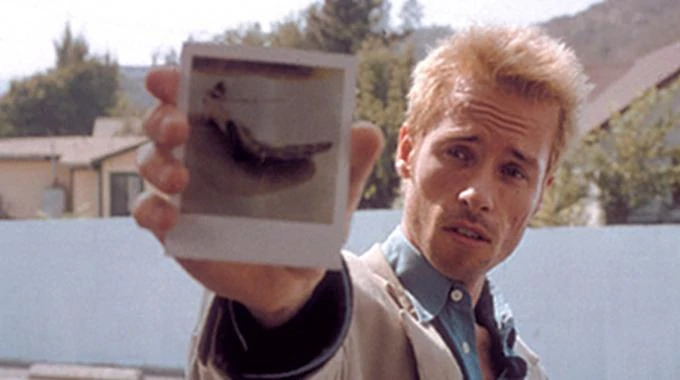
\includegraphics[width=\paperwidth,height=\paperheight]{images/leonard}}
\end{frame}

\begin{frame}{temperature}
	\begin{itemize}
		\item Is the "entropy" of a model's response
		\pause
		\item Low temperature tends to hew towards predictability and repetitiveness
		\pause
		\item High temperatures make models get...goofy. 
	\end{itemize}
\end{frame}

\begin{frame}{Training}
	\begin{itemize}
		\item Usually done on text corpuses
		\pause
		\item The Pile (825GiB), Github, ShareGPT, etc.
		\pause
		\item (cough) books3, others
		\pause
		\item And other terms like RLHF (Reinforcement Learning from Human Feedback)
		\pause
		\item The larger the model, the more resources it takes to train or re-train.
	\end{itemize}
\end{frame}

\begin{frame}{Parameters}
	\begin{itemize}
		\item Roughly corresponds to how "Complex" or "Smart" a model is.
		\pause
		\item (...very roughly)
		\pause 
		\item But \textit{definitely} correlates to resources needed to run the model.
		\pause
		\item Which is why, say, GPT-4 requires this....
	\end{itemize}
\end{frame}



\begin{frame}[plain]
	\makebox[\linewidth]{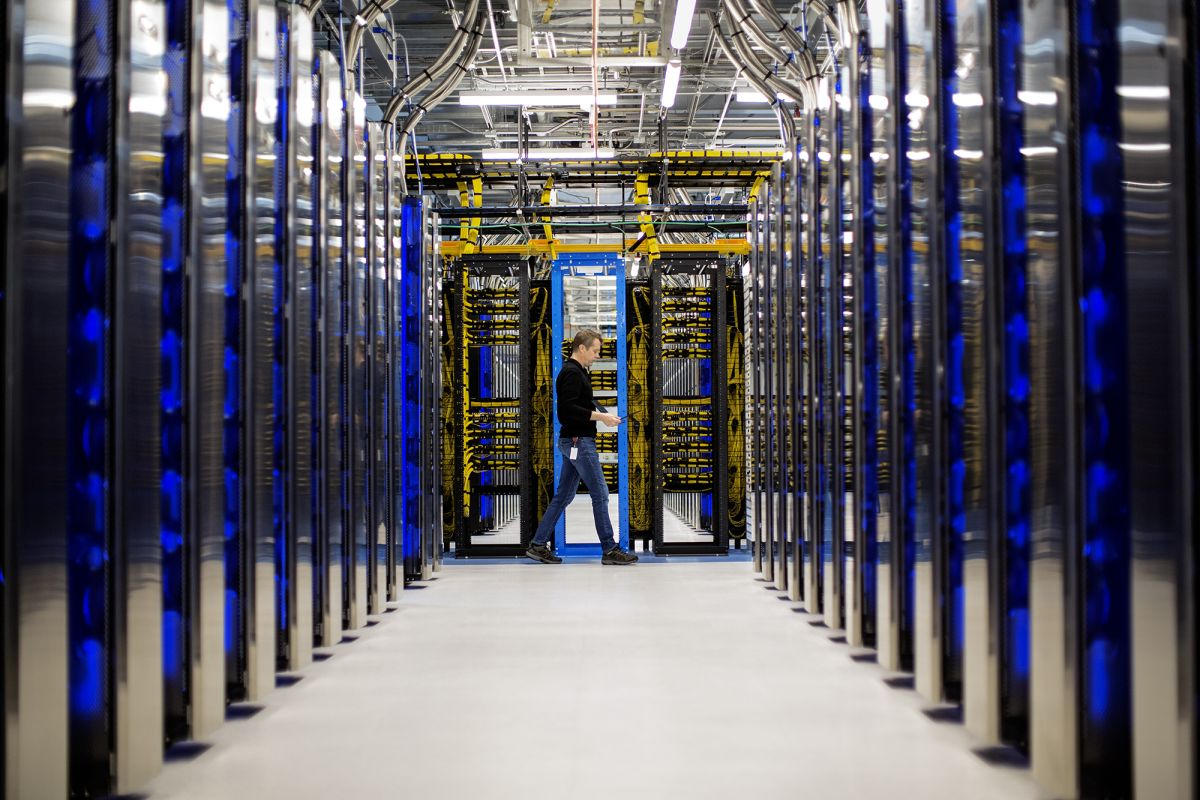
\includegraphics[width=\paperwidth,height=\paperheight]{images/azure-data-centre}}
\end{frame}

\begin{frame}
	And you can run a 7B model on this....
\end{frame}



\begin{frame}[plain]
	\makebox[\linewidth]{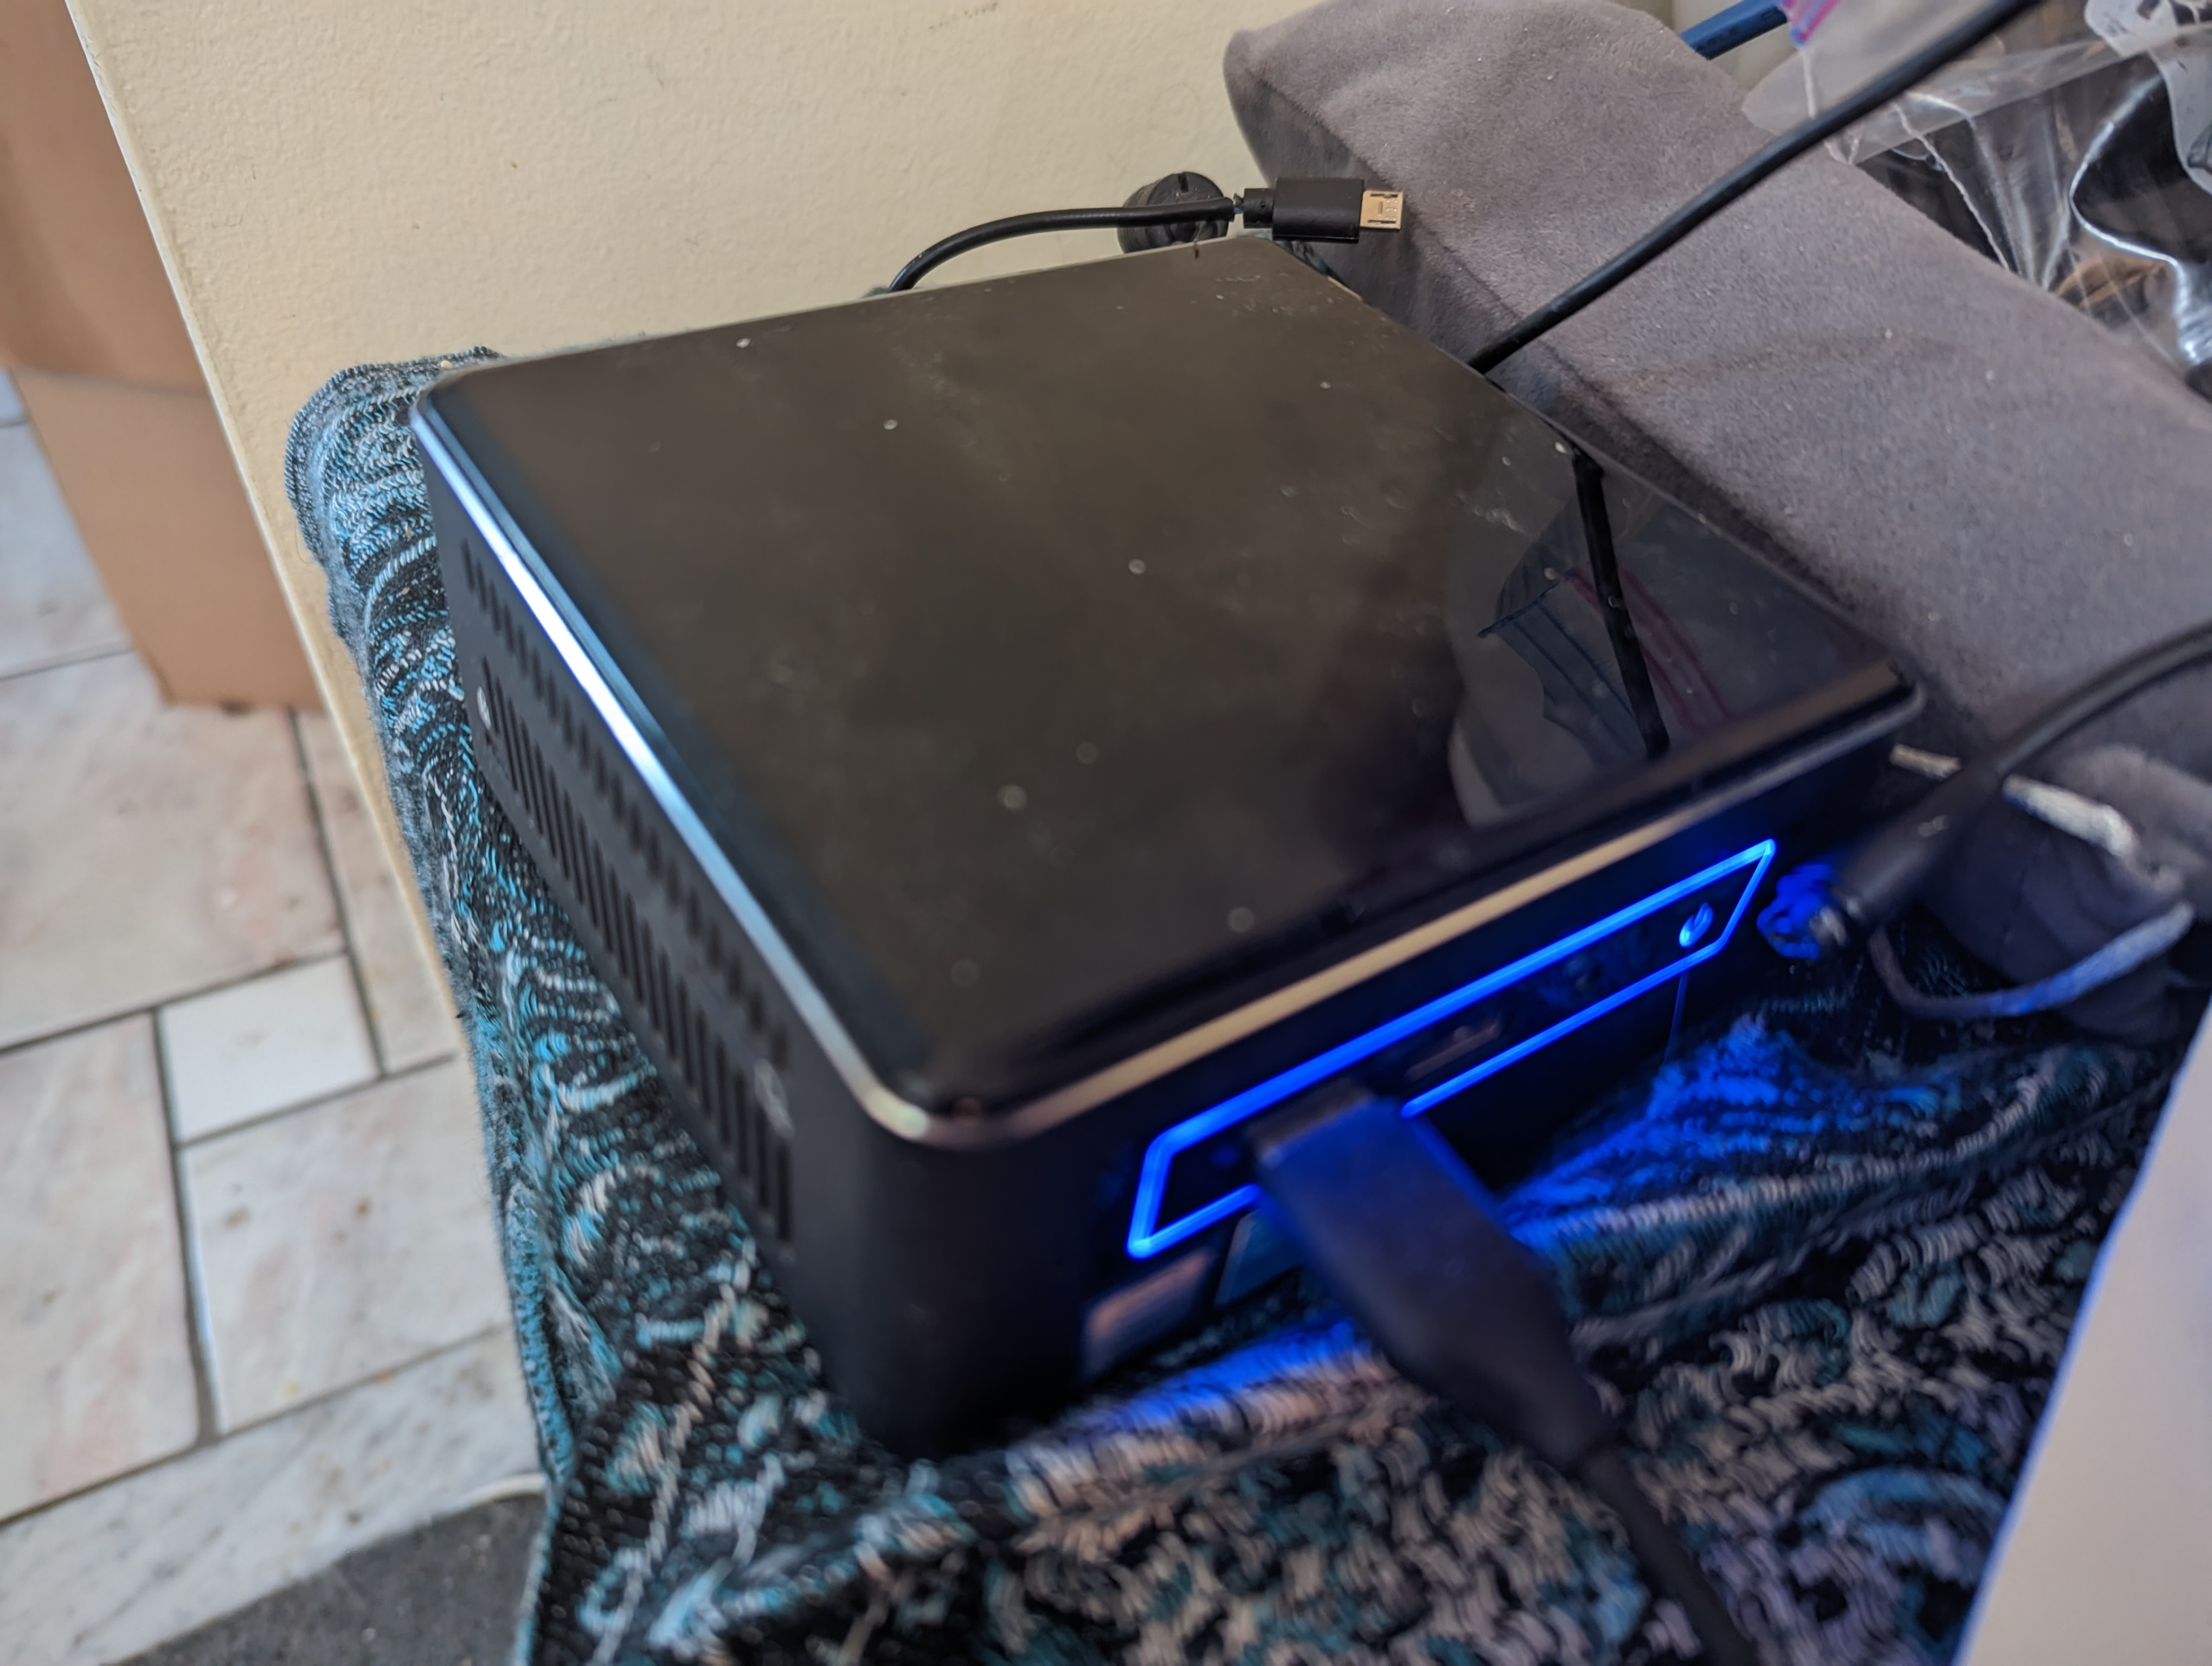
\includegraphics[width=\paperwidth,height=\paperheight]{images/pfeebe}}
\end{frame}

\begin{frame}
	And models get even smaller. Good (or at least amusing) results can be had from 1B and 0.5B parameters!
\end{frame}

\begin{frame}{what is \textit{quantization}}
	\begin{itemize}
		\item Consider TIFF files vs jpegs or FLACs vs mp3s
		\pause
		\item It's a way to *drastically* reduce compute needs at the expense of some level of fidelity
		\pause
		\item Without quantization, you pretty much need big GPUs -- 16GB Nvidias seem to be the base level
		\pause
		\item Quantized models \textit{can} use GPUs, and indeed function better if they do, but they don't \textit{need} them
	\end{itemize}
\end{frame}

\end{document}
